\chapter{Curvature, Contraction, and the Newtonian Limit}

This chapter follows Leonard Susskind's eighth lecture on general relativity. We begin where the previous lecture stopped: curvature shows itself when a vector is parallel transported around a small loop and fails to return to itself. The lecture then makes a deliberate turn toward operator language, because that is the economical way to derive the curvature tensor without drowning in notation. In the second half the emphasis changes just as sharply. Having built the tensors of curvature, we ask how they connect to the Newtonian picture of gravity as an acceleration field. The preserved board figures, kept here as documentary support from the lecture record associated with Leonard Susskind and documented through LazyingArt LLC and Video2Book, are used only where the board layout itself carries part of the argument.

\section{Curvature Revisited}

We begin with the geometric fact from the previous lecture. Take a small closed loop in space or spacetime. Parallel transport a vector around it. If the geometry is curved, the vector returns to the starting point with a slightly different orientation. The failure to come back to itself is the signal of curvature.

Susskind's point at the start of this lecture is that there is a fast way to derive the formula for that failure. The price is a little abstract notation, but it is notation of a familiar kind: operators acting on functions. Once we say this clearly, the central idea almost announces itself. Curvature will emerge as a commutator.

\section{Covariant Derivatives as Operators}

Let us take a vector field with components \(V^\alpha(x)\). We may think of it simply as a collection of functions of position. Then there are three natural kinds of operators that can act on it.

First, there is differentiation:
\begin{equation}
\partial_\mu V^\alpha(x).
\end{equation}

Second, there is multiplication by an ordinary function \(F(x)\):
\begin{equation}
F(x)\,V^\alpha(x).
\end{equation}

Third, there is multiplication by a matrix:
\begin{equation}
(MV)^\alpha = M^\alpha{}_\beta V^\beta.
\end{equation}

The important step is that the covariant derivative combines these into a single operator. In components,
\begin{equation}
(\nabla_\mu V)^\alpha
=
\partial_\mu V^\alpha
+
\Gamma^\alpha{}_{\mu\beta}V^\beta.
\end{equation}
For each fixed \(\mu\), the Christoffel symbols \(\Gamma^\alpha{}_{\mu\beta}\) can be viewed as the entries of a matrix \(\Gamma_\mu\). In that compact operator language,
\begin{equation}
\nabla_\mu = \partial_\mu + \Gamma_\mu.
\end{equation}

This is the first real simplification of the lecture. The Christoffel symbols are no longer just a messy three-index object. They are, for each \(\mu\), a position-dependent matrix acting on the vector components. That is the viewpoint that makes the curvature calculation fit on the board.

\section{The Commutator Trick}

Before the geometry returns, Susskind pauses for one small lemma. If \(F(x)\) is regarded as the operator of multiplication by \(F\), then
\begin{equation}
[\partial_x,F(x)] = \frac{dF}{dx}.
\end{equation}
The meaning of this is best seen by letting the commutator act on a test function \(V(x)\):
\begin{align}
[\partial_x,F]V
&=
\partial_x(FV)-F(\partial_xV) \\
&=
\frac{dF}{dx}V + F\frac{dV}{dx} - F\frac{dV}{dx} \\
&=
\frac{dF}{dx}V.
\end{align}
So the entire effect of the commutator is just multiplication by the derivative of \(F\). This is the one small technical theorem the lecture needs later.

The reason for introducing it now is very precise. Once we expand a commutator of covariant derivatives, we will meet terms in which an ordinary derivative stands next to a position-dependent matrix \(\Gamma_\mu(x)\). The lemma tells us exactly how to simplify those terms.

\begin{figure}[htbp]
\centering
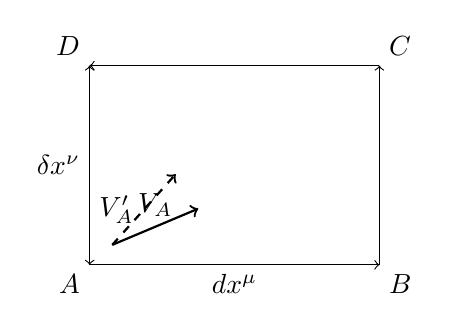
\begin{tikzpicture}[scale=1.15]
\draw[->] (0,0) -- (3.2,0) node[midway,below] {$dx^\mu$};
\draw[->] (0,0) -- (0,2.2) node[midway,left] {$\delta x^\nu$};
\draw[->] (3.2,0) -- (3.2,2.2);
\draw[->] (3.2,2.2) -- (0,2.2);
\draw[->] (0,2.2) -- (0,0);

\node[below left] at (0,0) {$A$};
\node[below right] at (3.2,0) {$B$};
\node[above right] at (3.2,2.2) {$C$};
\node[above left] at (0,2.2) {$D$};

\draw[->,thick] (0.25,0.22) -- (1.2,0.62) node[midway,above] {$V_A$};
\draw[->,thick,dashed] (0.25,0.22) -- (0.95,1.00) node[midway,left] {$V_A'$};
\end{tikzpicture}
\caption{Schematic reconstruction of the infinitesimal loop \(A\to B\to C\to D\to A\). The vector returns to the same point, but in general not with the same orientation.}
\end{figure}

Now we return to the geometric picture. Pick two infinitesimal displacements, \(dx^\mu\) and \(\delta x^\nu\). They span a small loop. Start with a vector \(V_A\) at the point \(A\), transport it around the loop \(A\to B\to C\to D\to A\), and call the returned vector \(V_A'\). The mismatch \(V_A-V_A'\) is what curvature must measure.

The lecture does not jump directly to the answer. Instead it engineers a difference of differences:
\begin{equation}
\big[(V_C-V_D)-(V_B-V_A)\big]
-
\big[(V_C-V_B)-(V_D-V_A')\big]
=
V_A - V_A'.
\end{equation}
This is the blackboard version of a second derivative. One first takes a difference in one direction, then compares that difference after shifting in the other direction; then one repeats the process in the opposite order and subtracts.

\subsection{Question \& Answer}

Why this particular combination? The lecture is very explicit: it is engineered. Susskind chooses the signs so that the interior terms cancel and the only survivor is the quantity he wants, namely the mismatch between the initial vector and the returned one. Had he chosen the opposite orientation conventions, the result would differ only by an overall sign. Nothing deep is hiding there; the combination is designed to isolate the loop effect.

What goes to zero when the loop shrinks? Not the Riemann tensor itself. What goes to zero is the actual change in the vector. The quantity \(V_A-V_A'\) is proportional to the small area enclosed by the loop, so it is doubly small in the two edge lengths. The curvature tensor is the coefficient of that area dependence. This is why it is better, at this stage, to write the result as a small change \(\Delta V\) rather than divide too quickly by the area and pretend we have an ordinary second derivative of some scalar.

Replacing the finite differences by covariant derivatives, we are led to
\begin{equation}
\Delta V
=
\big(\nabla_\nu\nabla_\mu - \nabla_\mu\nabla_\nu\big)V\,
\delta x^\nu dx^\mu
=
[\nabla_\nu,\nabla_\mu]V\,\delta x^\nu dx^\mu.
\end{equation}
This is the decisive bridge from geometry to algebra.

Now we expand the commutator. Using \(\nabla_\mu=\partial_\mu+\Gamma_\mu\),
\begin{align}
[\nabla_\nu,\nabla_\mu]
&=
[\partial_\nu+\Gamma_\nu,\partial_\mu+\Gamma_\mu] \\
&=
[\partial_\nu,\Gamma_\mu]-[\partial_\mu,\Gamma_\nu]+[\Gamma_\nu,\Gamma_\mu] \\
&=
\partial_\nu\Gamma_\mu-\partial_\mu\Gamma_\nu+\Gamma_\nu\Gamma_\mu-\Gamma_\mu\Gamma_\nu.
\end{align}
The pure derivative term disappears because ordinary partial derivatives commute. The mixed terms become derivatives of \(\Gamma\) by the commutator lemma. The last term survives because the \(\Gamma_\mu\) are matrices, and matrices need not commute.

Restoring the hidden matrix indices, the coefficient of \(V^\beta\) is the Riemann tensor. In standard component form,
\begin{equation}
R^\alpha{}_{\beta\mu\nu}
=
\partial_\mu \Gamma^\alpha{}_{\nu\beta}
-
\partial_\nu \Gamma^\alpha{}_{\mu\beta}
+
\Gamma^\alpha{}_{\mu\delta}\Gamma^\delta{}_{\nu\beta}
-
\Gamma^\alpha{}_{\nu\delta}\Gamma^\delta{}_{\mu\beta}.
\end{equation}
Thus the infinitesimal loop law becomes
\begin{equation}
\Delta V^\alpha
=
R^\alpha{}_{\beta\mu\nu}\,V^\beta\,\delta x^\nu dx^\mu.
\end{equation}

Suppressing the matrix indices, the cleanest mnemonic is that curvature is the commutator of covariant derivatives:
\begin{equation}
R_{\mu\nu}\sim[\nabla_\mu,\nabla_\nu],
\end{equation}
with the understanding that the suppressed indices are the matrix indices carried by the vector being acted upon.

\section{Symmetries, Contractions, and Lower-Rank Curvature}

Once the Riemann tensor is on the board, the lecture slows down and reads structure off from it. Lowering the first index with the metric gives the fully covariant tensor \(R_{\nu\mu\alpha\beta}\). In that form the lecture emphasizes three symmetries:
\begin{equation}
R_{\nu\mu\alpha\beta} = - R_{\mu\nu\alpha\beta},
\qquad
R_{\nu\mu\alpha\beta} = - R_{\nu\mu\beta\alpha},
\qquad
R_{\nu\mu\alpha\beta} = R_{\alpha\beta\nu\mu}.
\end{equation}
The first antisymmetry is immediate from the commutator construction. The second is stated in the lecture and tied to the fact that parallel transport preserves the length of the vector. The third is the pair-exchange symmetry of the fully lowered tensor.

The lecture also stresses what kind of object this is. Each Christoffel symbol contains first derivatives of the metric, so the Riemann tensor contains second derivatives of the metric and quadratic products of first derivatives. In that sense it is exactly the sort of object one expects to appear in a field equation for gravity.

\begin{figure}[htbp]
\centering

\includegraphics[width=0.55\textwidth]{lecture_08_figure_02.png}
\caption{Ricci-contraction notation on the board. The isolated expression is useful evidence for the contraction pattern, even though the exact mixed-index placement is better written in clean standard notation.}
\end{figure}

Now the lecture turns to a guided search. What lower-rank tensors can be made from the Riemann tensor?

If we contract the antisymmetric pair \(\mu,\nu\) with the symmetric metric, we get zero:
\begin{equation}
g^{\mu\nu}R_{\mu\nu\alpha\beta}=0.
\end{equation}
The same is true if we contract the antisymmetric pair \(\alpha,\beta\):
\begin{equation}
g^{\alpha\beta}R_{\mu\nu\alpha\beta}=0.
\end{equation}
So the only interesting contraction is a mixed one, taking one index from the first antisymmetric pair and one from the second. This defines the Ricci tensor:
\begin{equation}
R_{\mu\beta}
=
R^\alpha{}_{\mu\alpha\beta}
=
g^{\alpha\nu}R_{\nu\mu\alpha\beta}.
\end{equation}
The lecture then notes that \(R_{\mu\beta}\) is symmetric. Contracting once more gives the curvature scalar:
\begin{equation}
R = g^{\mu\nu}R_{\mu\nu}.
\end{equation}

Here Susskind is careful not to let the scalar do more work than it should. If \(R\neq 0\), the space is certainly curved. But \(R=0\) does not, in general, imply flatness. The lecture makes the dimension-dependent point only briefly: in two dimensions the scalar already controls flatness; in three dimensions the Ricci tensor does; in higher dimensions neither one by itself is enough, and one must really look at the full Riemann tensor.

There is also an important conceptual reminder at this point. The curvature under discussion is intrinsic curvature. One can bend a sheet of paper in an ambient space and still have zero intrinsic curvature. What the Riemann tensor measures is not how a surface sits in a higher-dimensional space, but what is felt by someone moving within the space itself.

\section{Slow Geodesics and the Newtonian Potential}

The second half of the lecture begins by changing the target. We no longer ask only what curvature is. We ask how general relativity reduces to Newtonian gravity when fields are weak and motions are slow.

The equation of motion is the geodesic equation:
\begin{equation}
\frac{d^2 x^\mu}{d\tau^2}
+
\Gamma^\mu{}_{\sigma\lambda}
\frac{dx^\sigma}{d\tau}
\frac{dx^\lambda}{d\tau}
=
0,
\end{equation}
with proper time defined by
\begin{equation}
d\tau^2 = g_{\mu\nu}\,dx^\mu dx^\nu.
\end{equation}
Now assume
\begin{equation}
g_{\mu\nu} = \eta_{\mu\nu}+h_{\mu\nu},
\qquad
|h_{\mu\nu}|\ll 1,
\end{equation}
and work in a frame in which everything moves slowly and changes slowly in time. Then \(x^0=t\) is approximately the same as \(\tau\), so
\begin{equation}
\frac{dx^0}{d\tau}\approx 1,
\qquad
\frac{dx^i}{d\tau}\ll 1.
\end{equation}
For the \(x\)-component of the geodesic equation, the dominant Christoffel term is therefore the one with two zero indices:
\begin{equation}
\frac{d^2x}{dt^2} \approx -\Gamma^x{}_{00}.
\end{equation}

Now expand the Christoffel symbol:
\begin{align}
\Gamma^x{}_{00}
&=
\frac12 g^{x\rho}
\big(
\partial_0 g_{\rho 0}
+
\partial_0 g_{0\rho}
-
\partial_\rho g_{00}
\big) \\
&\approx
\frac12 g^{xx}
\big(
2\,\partial_0 g_{x0}
-
\partial_x g_{00}
\big).
\end{align}
In the Newtonian regime the time derivatives are negligible, and \(g^{xx}\approx \eta^{xx}=-1\). Thus
\begin{equation}
\frac{d^2x}{dt^2}
\approx
-\frac12\,\frac{\partial g_{00}}{\partial x}.
\end{equation}

Newtonian gravity would have written the same acceleration as
\begin{equation}
\frac{d^2x}{dt^2} = -\frac{\partial\phi}{\partial x}.
\end{equation}
Comparing the two, we see the structure immediately: \(g_{00}\) is tied to the Newtonian potential. The lecture is openly unstable on signs at this point, and it is best to preserve that fact rather than hide it. What survives the sign confusion is the robust relation
\begin{equation}
g_{00}=2\phi+c,
\end{equation}
where the constant is fixed by the requirement that far from gravitating matter the metric approach the Minkowski form. In that limit \(g_{00}\to 1\), so the constant is eventually \(c=1\), though the lecture does not pause here to make that normalization the main point.

\begin{figure}[htbp]
\centering

\includegraphics[width=0.55\textwidth]{lecture_08_figure_03.png}
\caption{Newtonian acceleration and the boxed metric-potential relation on the board. The lecture wavers on signs here, but the boxed relation marks the intended takeaway.}
\end{figure}

The important conclusion is not yet the exact sign. It is that the time-time component of the metric is already carrying the Newtonian potential, up to a constant and a factor of two. That is the bridge from geodesics to gravity.

\section{Poisson's Equation and the Source \(T^{00}\)}

Having related \(\phi\) to \(g_{00}\), the lecture goes back to Newton and asks how the potential is tied to its sources. The board first writes the acceleration field \(A\), then its divergence law, then Poisson's equation. The exact sign tying \(A\) to \(\nabla\phi\) wobbles in the spoken derivation, but the stable structural point is the Poisson equation itself.

\begin{figure}[htbp]
\centering

\includegraphics[width=0.52\textwidth]{lecture_08_figure_04.png}
\caption{Newtonian gravity equations for the potential. The vertical stack on the board mirrors the lecture's move from acceleration field to divergence law to Poisson equation.}
\end{figure}

In cleaned form we may write the Newtonian source equations as
\begin{equation}
\nabla\cdot A = -4\pi G\rho,
\qquad
\nabla^2\phi = 4\pi G\rho,
\end{equation}
where
\begin{equation}
\nabla^2\phi
=
\frac{\partial^2\phi}{\partial x^2}
+
\frac{\partial^2\phi}{\partial y^2}
+
\frac{\partial^2\phi}{\partial z^2}.
\end{equation}

Now comes the relativistic rewriting. In units with \(c=1\), mass density is energy density. And energy density is the \(00\)-component of the energy-momentum tensor. So the Newtonian source equation becomes
\begin{equation}
\nabla^2\phi = 4\pi G T^{00}.
\end{equation}
Using \(\phi=\tfrac12 g_{00}\), we obtain
\begin{equation}
\nabla^2 g_{00} = 8\pi G T^{00}.
\end{equation}

\begin{figure}[htbp]
\centering

\includegraphics[width=0.60\textwidth]{lecture_08_figure_05.png}
\caption{Poisson equation rewritten with \(T^{00}\). The lower line makes the weak-field bridge from the Newtonian potential to \(g_{00}\).}
\end{figure}

This is the first genuinely suggestive equation of the second half of the lecture. It tells us that, at least in a slow-moving weak-field frame, the energy density determines the second spatial derivatives of \(g_{00}\). In other words, matter is beginning to tell the metric what to do.

\section{Toward a Tensor Equation}

At this point the lecture turns the result against itself. What is wrong with the equation
\[
\nabla^2 g_{00} = 8\pi G T^{00}?
\]
Nothing is wrong with it as an approximation in the frame where we derived it. The problem is that it is not yet a tensor equation. It is a statement about one component of the metric in a special frame. General relativity, however, must be written in a form that holds in every frame.

The right-hand side is already a component of a tensor. The board emphasizes this by sketching the beginning of the stress-energy layout.

\begin{figure}[htbp]
\centering

\includegraphics[width=0.72\textwidth]{lecture_08_figure_06.png}
\caption{Weak-field equation beside the first stress-energy entries. The split-board layout records the lecture's transition from scalar weak-field reasoning to the search for a full tensor equation.}
\end{figure}

The corresponding mathematical picture is
\begin{equation}
T^{\mu\nu}\sim
\left(
\begin{array}{ccc}
T^{00} & T^{01} & \cdots \\
T^{10} & T^{11} & \cdots \\
\vdots & \vdots & \ddots
\end{array}
\right).
\end{equation}
So the left-hand side must also be a two-index tensor, built only from the metric and its derivatives, and in the weak-field limit its \(00\)-component must reduce to the equation we have just obtained.

What two-index tensors are available? By this point in the lecture the answer is almost forced. The natural candidates are the Ricci tensor \(R_{\mu\nu}\) and the metric times the scalar curvature, \(g_{\mu\nu}R\). Therefore the most general candidate at this level is
\begin{equation}
A\,R_{\mu\nu}+B\,g_{\mu\nu}R=8\pi G\,T_{\mu\nu},
\end{equation}
for some numerical constants \(A\) and \(B\).

This is exactly where the lecture stops. Susskind even gives away, as a teaser, that the coefficients will turn out to be \(1\) and \(-\tfrac12\). But he does not derive that here, and one should not smooth away that incompletion. The real achievement of this lecture is to set the target with clarity. The gravitational field must be a tensor made from second derivatives of the metric, and in the Newtonian limit it must reproduce the weak-field equation for \(g_{00}\).

\section{Summary}

The lecture begins with the geometric fact that curvature is measured by the failure of a vector to return to itself after transport around a small loop. It then converts that fact into algebra by treating covariant derivatives as operators and computing their commutator. From this we obtain the Riemann tensor, read off its symmetries, and contract it to the Ricci tensor and curvature scalar.

The second half asks for the Newtonian meaning of these constructions. In the weak-field, slow-motion regime, the geodesic equation reduces to ordinary acceleration, and the comparison with Newtonian gravity ties \(g_{00}\) to the potential \(\phi\). Poisson's equation then becomes a weak-field relation between \(g_{00}\) and \(T^{00}\). The lecture ends exactly where it should end: not with Einstein's equation fully derived, but with the sharply posed question of what tensor built from the metric can replace that weak-field component equation in every frame.